\documentclass[11pt,a4paper]{report}
\usepackage[hmargin=1.25in,vmargin=1in]{geometry}
\usepackage{amsthm}
\usepackage{cite,url,amsmath,amssymb,bm}
\usepackage{algorithm,graphicx,color,mathtools}
\usepackage{physics,enumitem,thmtools}
\usepackage{hyperref}


\title{The Solution of Model Predictive Control: Theory, Computation, and Design}
\author{lixc21}
\date{\today}



\newtheorem*{remark}{Remark}
\theoremstyle{definition}\newtheorem{exercise}{Exercise}[chapter]
\declaretheoremstyle[
  headfont=\color{blue}\normalfont\bfseries,
  bodyfont=\color{blue}\normalfont,
]{colored}
\declaretheorem[
  style=colored,
  name=Answer,
]{answer}



\begin{document}
\maketitle

\chapter{Getting Started with Model Predictive Control}
\section{Brief Review}
In this section, we just consider state space linear time invariant system with zero steady state.

\paragraph{Lemma 1.3} (LQR convergence). For $(A,B)$ controllable, the infinite LQR gives a convergent closed-loop system.
\begin{proof}
Because $(A,B)$ is controllable, there exists a sequence of $n$ inputs that transfers the state to zero. When $k>n$, we let $u=0$, then the objective function $V(x,u)=\sum_{k=0}^\infty x_k^\top Qx_k+u^\top Ru$ is finite, which implies the optimization problem is feasible. On the other hand, the solution is unique since $R>0$ and the objective function is strict convex with $u$.

So the solution of the LQR problem exists and is unique. This implies to that the objective function is non-increasing with time, and we have $x\to 0$, $u\to 0$ as $k\to 0$.
\end{proof}
\begin{remark}
The optimal solution can be calculate from Riccati equation, which is from backward dynamic programming similar to Kalman filter.
\begin{equation}\notag
\begin{aligned}
K&=-(B^\top PB+R)^{-1} B^\top PA\\
P&=Q+A^\top PA-A^\top PB(B^\top PB+R)^{-1}B^\top PA
\end{aligned}
\end{equation}
\end{remark}


\section{The Solution of Exercises}
\begin{exercise} State space form for chemical reaction model.\\
Consider the following chemical reaction kinetics for a two-step series reaction
\begin{equation}
    A\xrightarrow{k_1} B\qquad B\xrightarrow{k_2} C
\end{equation}
We wish to follow the reaction in a constant volume, well-mixed, batch reactor. As taught in the undergraduate chemical engineering curriculum, we proceed by writing material balances for the three species giving
\begin{equation}
    \dv{c_A}{t}=-r_1\qquad \dv{c_B}{t}=r_1-r_2\qquad \dv{c_C}{t}=r_2
\end{equation}
in which $c_j$ is the concentration of species $j$, and $r_1$ and $r_2$ are the rates $\rm (mol/(time\cdot vol))$ at which the two reactions occur. We then assume some rate law for the reaction kinetics, such as
\begin{equation}
    r_1=k_1 c_A\qquad r_2=k_2 c_B
\end{equation}
We substitute the rate laws into the material balances and specify the starting concentrations to produce three differentia equations for the three species concentrations. 

\begin{enumerate}[label=(\alph*)]
    \item write the linear state space model for the deterministic series chemical reaction model. Assume we can measure the component A concentration. What are $x$, $y$, $A$, $B$, $C$, and $D$ for this model?
    \item Simulate this model with initial conditions and parameters given by $$c_{A0}=1\quad c_{B0}=c_{C0}=0\quad k_1=2\quad k_2=1$$
\end{enumerate}
\end{exercise}

\begin{answer}
\begin{enumerate}[label=(\alph*)]
    \item the linear state space model is
    \begin{equation}
        \dv{x}{t} = 
        \begin{bmatrix}
            -k_1 &0 &0 \\
            k_1 &-k_2 &0 \\
            0 &k_2 &0 \\
        \end{bmatrix} x = A x
    \end{equation}
    where $x=[c_A,\ c_B,\ c_C]^\top$. $B$ does not exist because there is no system input variables. $C=[1,\ 0,\ 0]^\top$, $D=0$, $y=Cx$.
    
    \item the simulation result is shown as Fig.\ref{figans1}. The code used in all of the exercise can be found in github \url{https://github.com/lixc21/MPC-Solution}.
\end{enumerate}
\begin{figure}[htbp]
    \centering
    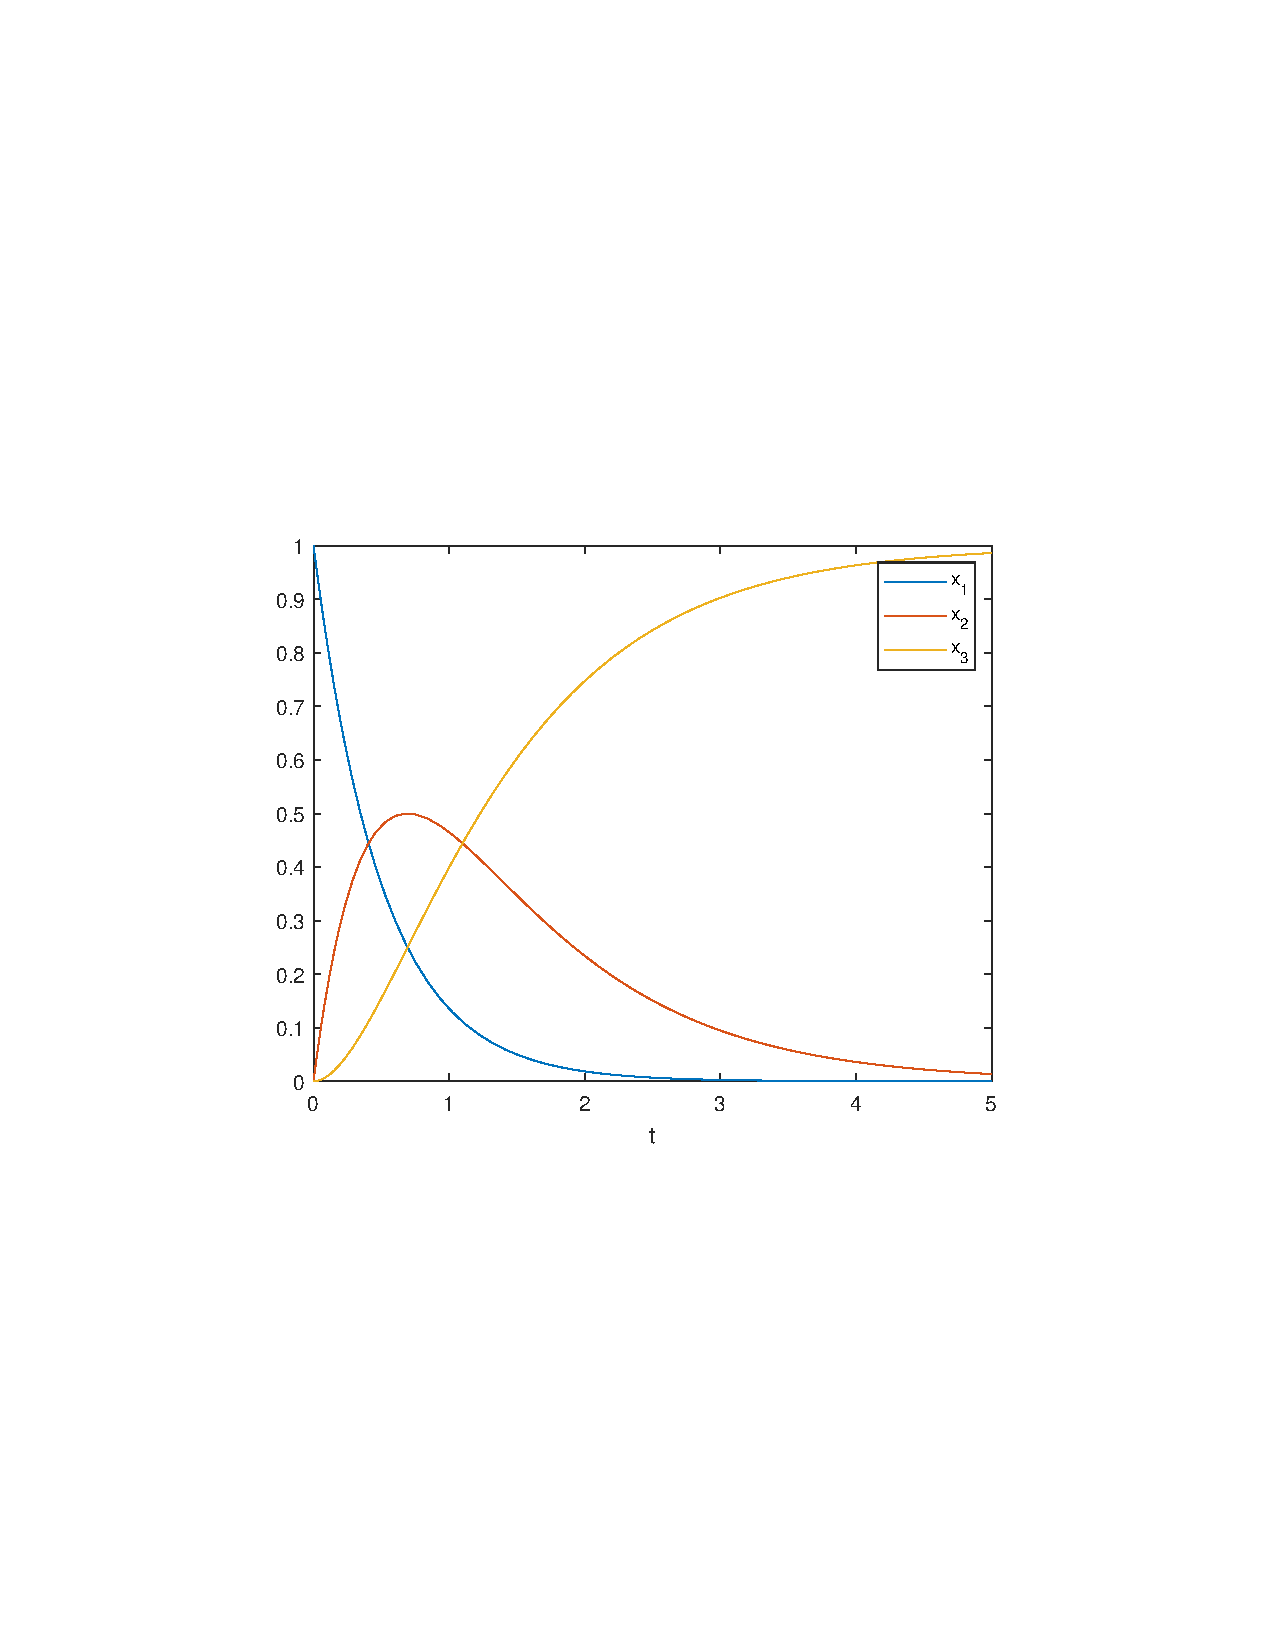
\includegraphics[width=\linewidth/2]{./code_ch1/exer1.pdf}
    \caption{system simulation}
    \label{figans1}
\end{figure}
\end{answer}

\begin{exercise}
    
\end{exercise}

















\chapter{Appendix A. Mathematical Background}
Since the mathematical background is basic, we jump to the exercises section.
\section{The solution of Exercises}
\begin{exercise} Norms in $\mathbb{R}^n$\\
Show that the following three functions are all norms in $\mathbb{R}^n$

\begin{equation}\notag
    \|x\|_2 
\end{equation}

\end{exercise}


\end{document}

























